\documentclass[a4paper]{llncs}
\usepackage{amsmath, amssymb}
%\usepackage{makeidx}  % allows for indexgeneration
\usepackage[pdftex]{graphicx} % PNGs
\usepackage[ngerman,english]{babel}
\usepackage[utf8x]{inputenc}
\usepackage[T1]{fontenc}
\usepackage{listings} % for sourcecode
\usepackage{graphviz} % graphs
\usepackage{array} % tables
\usepackage{afterpage} % figures
\usepackage{float} % figures
\usepackage{wrapfig} % figures im fließtext

%Smalltalk listings
\lstdefinelanguage{Smalltalk}{
  morekeywords={true,false,self,super,nil},
  sensitive=true,
  morecomment=[s]{"}{"},
  morestring=[d]',
  style=SmalltalkStyle
}
\lstdefinestyle{SmalltalkStyle}{
  %literate={:=}{{$\gets$}}1{^}{{$\uparrow$}}1{>>}{{\frqq}}1
  literate={^}{{$\uparrow$}}1{>>}{{\frqq}}1
}
\lstset{%
  	language=Smalltalk,
	basicstyle=\small,
	frame=lines,
	breaklines=true,
	%breakatwhitespace=false,
	captionpos=b,
}
%\newcommand{\trademark}{$^\text{\texttrademark}$~}
%\newcommand{\registered}{{$^\text{\textregistered}$}~}
\newcommand{\trademark}{\texttrademark~}
\newcommand{\registered}{\textregistered~}

% Ein beispiel Listing
%
%\begin{lstlisting}[language=Smalltalk]
%HelloWorld>>sayHelloTo: aString
%    "print a hello world message"
%    Transcript show: 'Hello, ', aString, '!'
%    name := 'a new name' "This is a comment"
%    ^ name
%\end{lstlisting}

\begin{document}
\nocite{*}
\mainmatter              % start of the contributions
\title{XO-Bubbles}
\subtitle{A Frozen Bubble Clone in Smalltalk/Squeak}
\date{\today}
\author{Tim Felgentreff, 738147}
\author{Konstantin Haase\inst{1}, Tim Felgentreff\inst{1}, Johannes Wollert\inst{1}, 
Michael Winkelmann\inst{2}, Robert Pfeiffer\inst{1}}

\institute{%
Hasso-Plattner-Institut, Universität Potsdam, D-14482 Potsdam, Germany,\\
\email{\{konstantin.haase,tim.felgentreff,johannes.wollert, robert.pfeiffer\}@student.hpi.uni-potsdam.de}
\and
Institut für Informatik, Universität Potsdam, D-14482 Potsdam, Germany,\\
\email{mwinkel@uni-potsdam.de}}

\maketitle

\begin{abstract}
  {With the rise of the Web 2.0 social networking sites, our social interactions
have gained another facet. As with every social activity, confinement
to a lone computer session thins out the user-group considerably.
If the social web is 
to persists this cannot be the end of the story. Yet, broad use of social networks on-the-go 
with the help of
the increasingly popular smartphones is held back by the large form factor of 
those devices, and the fact that they are not specialized to perform this 
task. In this paper, we propose a tiny mobile device tailored to the needs 
of the social web user. In our user study, participants were able to access
their most wanted features more quickly and with less error compared to a 
regular smartphone with a web browser.
}
\end{abstract}

%:= the shortest path between a commonly believed fact
%and the research question you are answering in your paper
%
%Example (Shift, CHI 2007)
%to save time for retrieving the stylus, users operate PDAs using touch
%finger tip size and occlusion make acquisition of small targets hard
% zooming does not fix that occlusion (see section “user test paper”)
% offset cursor solves the problem, but has three drawbacks
%we propose ‘Shift’. It solves the problem while avoiding the 3 drawbacks
%
%one paragraph for each logical step in that argument
%if you need more than, say, 6 paragraphs you are probably underestimating your audience and started too far back
%write in logical order, not in the chronological order in which you came up with it (this is not a diary)
%
\section{Introduction}
Social Web is the next logical extension to Mail and SMS to keep track of your associates. 
Social websites have gained much larger user bases than ``traditional'' web communities and demand
for new ways of access to the communities is high.
Traditionally, 
anything web-related was performed at a computer and only recently, with the wide-spread adoption of 
smartphones, the desire to use such networks ubiquitously emerged. Let's see how this is done today:
\begin{itemize}
  \item %
    Users usually 
    use the web browser of their smartphone system. This is the obvious solution for the inexperienced,
    and it is guaranteed to work with their social network of choice.
  \item Even with clever zooming techniques, the small screen is unsuitable for feature-packed sites such as Facebook\registered. 
    This alienates users. Still, they will likely not give up social networking, but rather look for a new 
    way of using it on-the-go
  \item Persistent users will soon find specialized apps for example on the Android\trademark platform or for the 
    Palm\registered Pre, however, 
    those apps still have to be started each time. Such delay, now matter how small, may offset users from doing what they were 
    trying to do completely, as users generally do not see the point of waiting 10 seconds for an application to start 
    only to see they do not have any new messages in their inbox.
\end{itemize}
To resolve those issues,we propose a specialized, small and unobtrusive device tailored towards a 
single purpose: to access the 
most used features of social networks in a consistent manner without delay or other 
inconvenience. We want social networking to
become the natural daily experience its users wanted it to be all along.
\begin{figure}[h]
  \begin{center}
    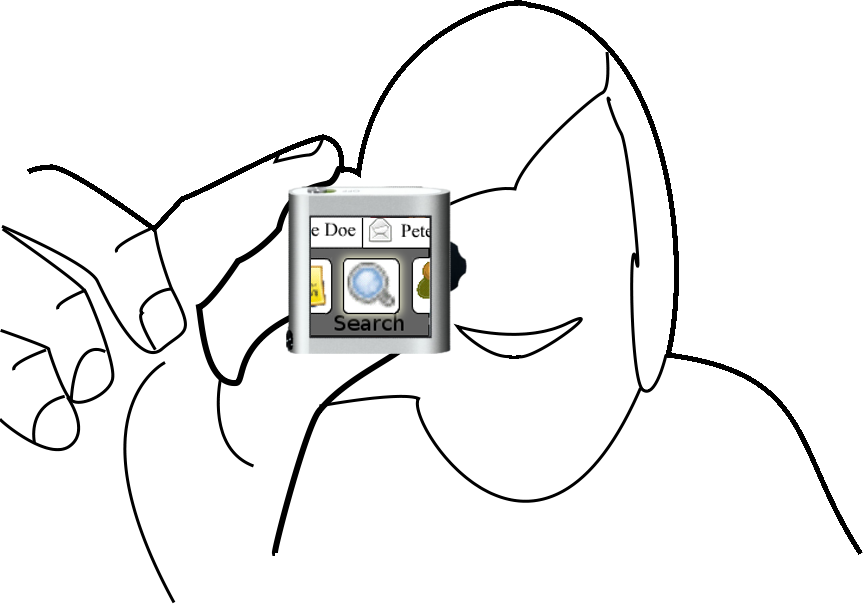
\includegraphics[width=0.8\linewidth]{imgs/main.png}
  \end{center}
  \caption{The SocioPath Device in Context}
  \label{fig:main}
\end{figure}

\section{Architecture}
In our system we have a set of classes which are central to the 
game. Those classes handle theming, player actions, game logic 
and the graphical representation of the game. These central
classes of our game are depicted in Fig.\ref{fig:architecture}.
%
The first instantiated class is FBGame. FBGame controls the game functionality, 
like the number of players, reward strategies like highscores and the
conditions of victory and defeat. FBGame is also responsible for instantiating
the FBWorld class which encapsulates graphical representation of the game.

FBWorld is passed a symbol at startup, which is resolved to a FBTheme. FBWorld 
holds a reference to the current theme and creates its main submorphs, like
a menu, highscore list the changing backgrounds and the in-game playfields.
These Morphs, however, are not held in an instance variable of any kind, but 
are returned to the FBGame instance, for co-ordination.\\
Out of technical necessity, FBWorld also catches all keytrokes, handling them, 
however, is up to the FBGame. Global events, like pause and quit, are handled 
directly, all other keystrokes are passed on to all playfields in the game (if any)
and handled there.

FBPlayfields are created by the world upon the requirements of the theme
and then returned to the FBGame. The playfields receive their own reference 
to the theme and are themselves responsible for their content and reaction on 
player input, thus allowing us to implement multiplayer gaming simply by creating 
more playfields in our world.
%
\begin{figure}[bt]
  \begin{center}
    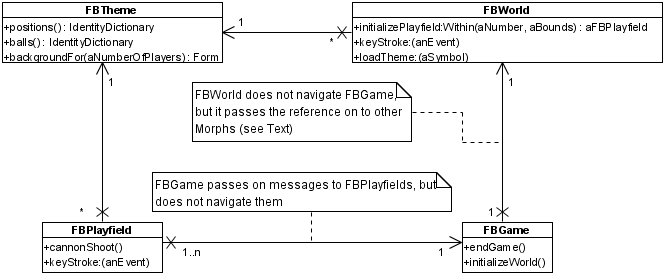
\includegraphics[width=0.6\linewidth]{images/architecture.png}
  \end{center}
  \caption{The central system architecture}
  \label{fig:architecture}
\end{figure}



\section{Design Process}
\subsection{Design Goals}
In order to achieve a pleasant and cleanly written FrozenBubble clone, we specified certain design goals.
A goal we set for ourselves very early was themeability, e.g. the ability to modify and 
adjust certain visual and logical aspects of the game (for example ball images or 
cannon positions). This demands an efficient and maintainable theme management 
system, as lots of pictures and data need to be processed.
As previously stated, another important aspect of our clone is ''realistic'' 
collision between objects, which came with certain performance considerations.
Lastly, we wanted our game to support multiplayer functionality. Given the time 
needed to implement networking, we decided to focus on a local multiplayer modes. 

\subsection{Slow Disk I/O}
%
Different from the original, we wanted to decouple the game from its representation 
to the point that we could allow different themes to change the positions of the 
game objects for different images and backgrounds. We decided to use png images to allow 
great visual flexibility and XML files to define the theme's positions. As disk I/O
is expensive, we needed a way to avoid it as much as possible, without sacrificing 
flexibility. Thus, lazy initialization for our FBTheme class was not an option. 
We created a class solely responsible for caching images and use the flyweight 
pattern to avoid reloading a theme we already loaded.
%
\subsection{Collision Between Balls}
\label{sec:collision}
When a ball is shot into the playfield, it has to interact with the plafield 
and other objects in its path. Simply looping over all those objects and 
testing for collision is in O(n) and result in slower 
movement of the ball and a general loss in responsiveness. A quick solution 
would have been to keep two lists of all objects sorted by their x and by their 
y axis, and only testing those items closest to the current ball in both lists.
Now O(n) would only be the worst case. 
It occured to us that using rasterization or using precalculated vectors similar 
to ray-tracing techniques could get us a constant complexity. We decided 
to implement rasterization, because it was a faster solution and allowed straight 
forward optimization.
%
\subsection{Falling Balls}
\label{sec:garbage}
When balls can collide and stick to each other, having them fall down 
if three or more of the same kind touch is trivial. However, balls 
hanging off balls that fall may have to fall as well. We considered 
two ways of checking for such conditions. We first planned to regard balls in the 
playfield as a network of nodes and use a graph search algorithm to determine 
whether or not a given ball has a connection to the top of the playfield via 
others. This proved difficult to implement and hurting encapsulation. Thus 
<<<<<<< HEAD:design.tex
we applied a metaphor of a garbage collector (GC) to the problem, where balls
ball that are not connected to the top are collected. Performance was no pressing 
concern here, as the number of balls in one playfield is relatively limited, 
and the algorithm runs at a moment where the user has just shot, so taking a second 
for the calculation would not hurt the game flow.
=======
we applied a metaphor of a garbage collector (GC) to the problem. First we used a
``reference counting GC'' where a ball registered itself with the balls he hung 
off. If any those balls fell, they reported to each registree so that they would 
decrement their reference count. If the reference count fell to zero, the ball 
would fall. However, this approach led to some problems with circular shapes 
in the playfield. Due to this we switched to a ``mark and sweep GC'' which traverses
over the balls in the field. Though this might sound less optimal performance-wise,
you have to keep in mind that the number of balls in one playfield is relatively limited, 
and also that the GC runs at a moment where the user cannot shoot anyway, so 
it is not time-critical.

\subsection{Simple Multiplayer Mode}
Several problems occured when we implemented a simple local multiplayer mode. In this chapter, 
we will discuss the most important design decissions.

%
  \paragraph{Players need to be informed of critical actions happening in other players' playfields}
    Direct communication between playfields would be the most simple solution like and 
    could be implemented easily. Additionally only the most rudimentary communication is needed,
    so there would be very few overhead. But this is not an object-oriented solution and playfields 
    would need to be hardcodedly enumerated, making the code hardly maintainable and badly extensible.\\
    In contrast, delegating communication through a mediator makes very maintainable and
    expandable code. Other than the previous proposal, this is indeed an object-oriented 
    take on the problem. However, there is more than twice as much communication happening 
    compared to the previous, simplified solution.\\
    Due to the obvious disadvantages of hardcoding different playfields, we chose the latter proposal.\\

  \paragraph{Different playfields have to be controlled by different players.
             And, of course, different playfields have to exist in the first place.}
    Our first idea we came up with was enabling the generic playfield to manage all needed behaviour
    on itself. That way, no new code needs to be introduced, rendering this scheme very simple.
    On the other hand, the playfield might have to be extended for all purposes to work properly. 
    This might lead to a very huge class indeed, affecting the readability.\\
    Introducing an Abstract Factory for playfields was another idea, thus implementing several 
    behavioural patterns. The obvious advantage of this proposal is, that Abstract Factories 
    are extensible and object-oriented. The downside of it would be, that this is a very powerful 
    pattern and would probably be overindulgence because we just need two different playfields 
    (single- and multiplayer behaviour). Because of that, we chose our initial idea of keeping 
    things simple.\\
%
\end{description}
%


\section{System Overview}
%
\begin{figure}[bt]
  \begin{center}
%    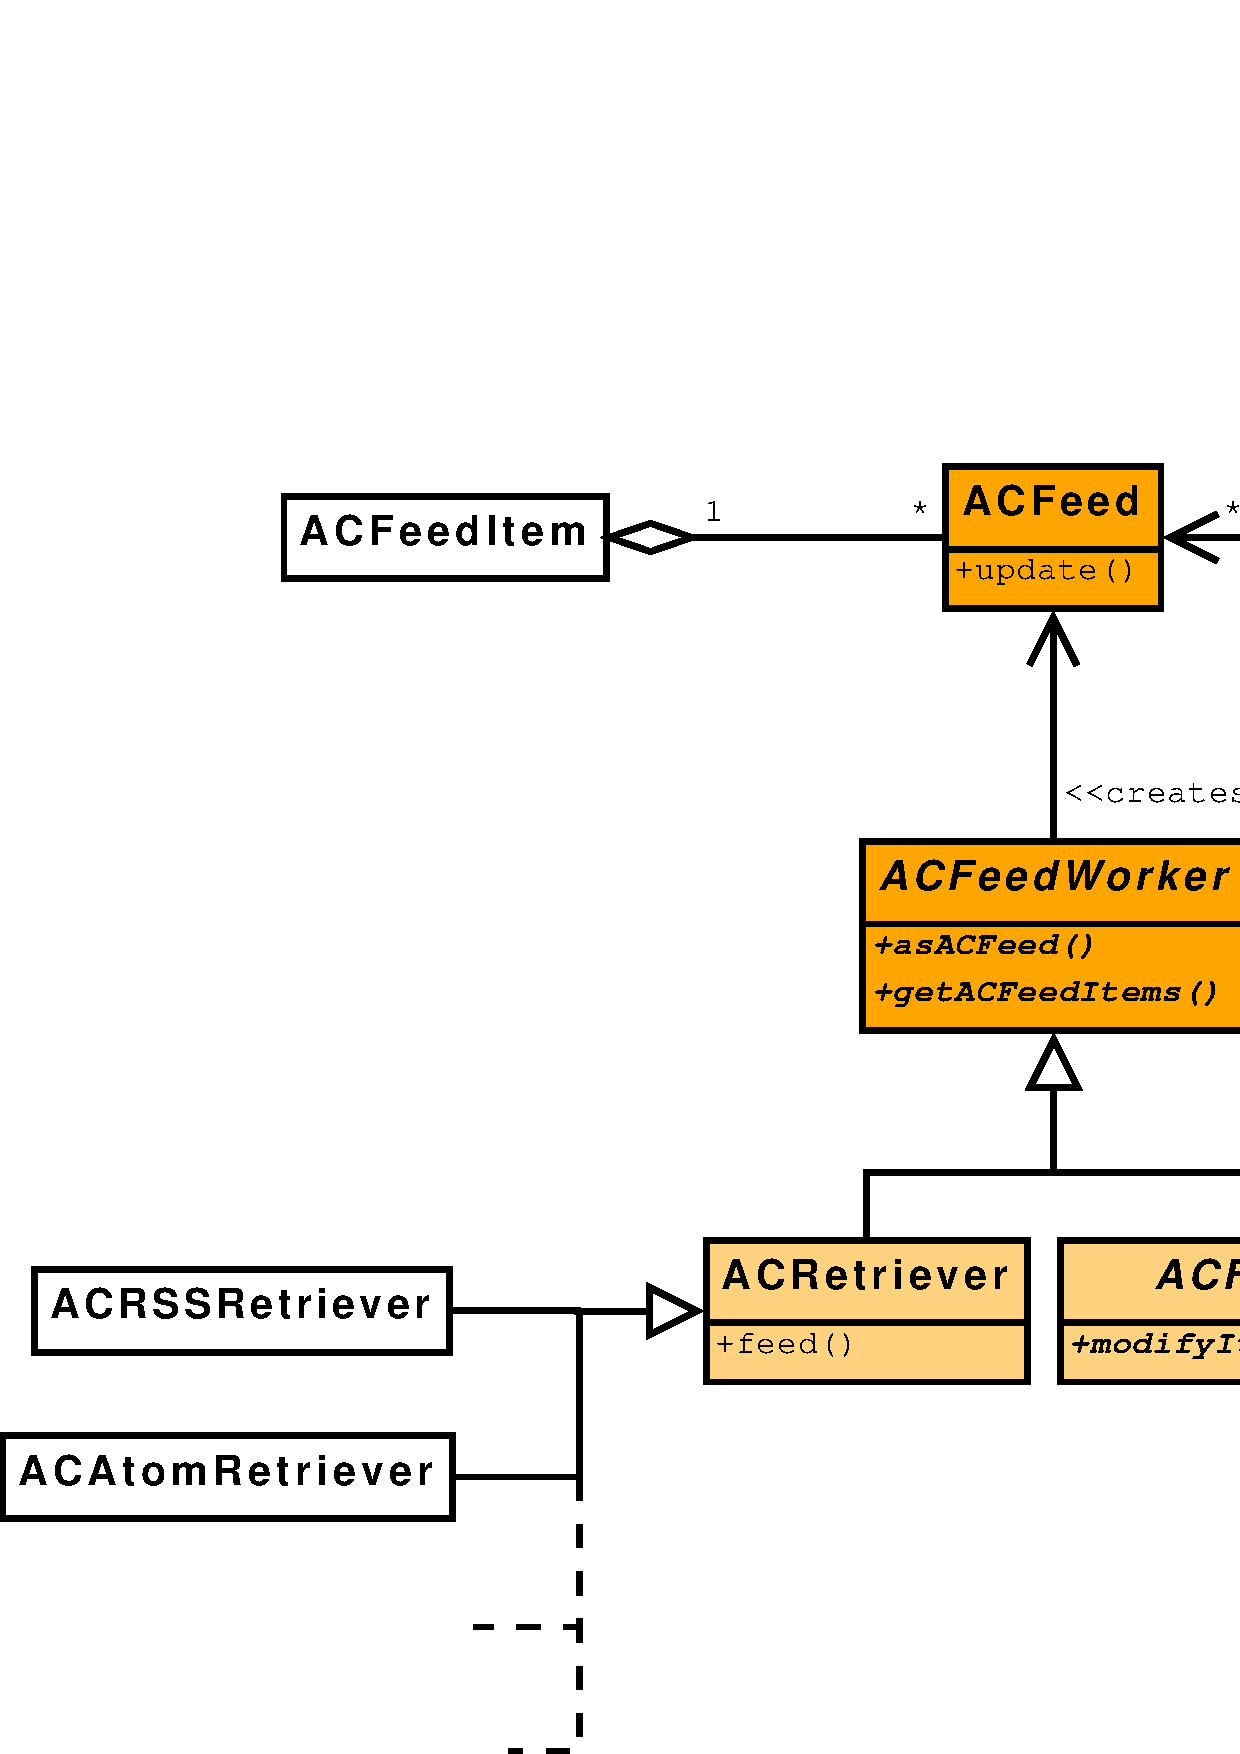
\includegraphics[width=0.9\linewidth]{images/system.png}
  \end{center}
  \caption{The complete system overview}
  \label{fig:system}
\end{figure}
%
\subsection{Interactions and Responsibilites}
\subsubsection{Themes and External Resources} ~\\
The FBTheme class is implemented as flyweight, holding references to previously 
created instances of a particular theme. If a requested theme type is not yet 
held in the list of instances, the class calls a builder class, 
FBThemeBuilder~\ref{fig:system}(1), to parse the requested theme's XML file, 
load the images and then return a fresh instance of the theme. Additionally, 
each theme contains an FBImageLibrary. The image library is just a simple 
wrapper around an IdentityDictionary to ease filling it with Forms. 
FBTheme and FBImageLibrary also support scaling to adjust to any screen 
size (without accounting for neccessary interpolation).
The FBImageLibrary is filled prior to starting the actual game, so 
that all external resources are cached. A lazily initialized image 
library would have resulted in slow disk I/O during
run-time.
\subsubsection{Rewarding the Players} ~\\
FBRewardStrategies are supporting classes which add rewarding behaviour 
to the game logic
~(Fig.\ref{fig:system}(2)). Its specializations 
implement different strategies to
reward the players for good gaming. Good gaming is measured by the 
number of balls falling, if more are falling at the same time, more 
reward points are gained.
The reward strategies have to implement a method
rewardPlayer:for:~\ref{lst:reward}.\\
In single player mode, a FBHighscoreReward
adds a simple highscore to the screen (responsible for adding the 
score visual is also the strategy itself) and for any number of 
reward points reported by the FBPlayfield, score points are accumulated.
%
\begin{lstlisting}[float,label=lst:reward,caption=The Highscore Calculation Method]
FBHighscoreReward>>rewardPlayer: aPlayer for: anAchievmentScalar
    "I reward a single player with an exponentially 
rising rate of points" 

    self score:
         self score + (anAchievmentScalar raisedTo: 2)
    \end{lstlisting}
%
In multiplayer mode, the strategie only rewards, if the player eliminates 
more than three balls from the field with a single shot. If that happens, 
a number of balls half as great is distributed among the other players,
and shot randomly in any direction. This happens via a call to 
the playfields which have to shoot random balls, since FBRewardStretegies
hold a collection referring to all playfields.
%
\subsubsection{Playfield Morphs} ~\\
As aforementioned, FBPlayfield is responsible for creating its own 
contents~\ref{fig:system}(3). Such content displays a cannon, a 
player avatar , messages for the user and numerous coloured balls. 
Each of these serves only a single, limited purpose, with FBPlayer 
and FBMessage merely wrapping different types of graphical response.
The cannon is the entity that reacts to the user's input, panning 
left and right and sending balls off into the field. However, it 
is controlled entirely by the playfield and does not act itself.

The FBBall is an exception to this simplicity. 
\begin{description}
  \item[First]
    	it has to look 
	differently, showing different colors in our themes. 
  \item[Secondly]
    	a Ball has different stages in its lifetime, being 
	loaded into the cannon, then flying, hanging from the 
	ceiling (or, indeed, from other balls) and finally falling 
	and vanishing.
  \item[Finally]
    	a Ball needs to collide with the playfield boundaries and 
	other balls in the field.
\end{description}
Thus its implementation is a bit larger, as it implements the FBCollider 
interface, utilizes different ``states'' to act on in its step method and 
and also draws itself from a collection of images.
%
\subsection{FBCollisionMap}
% \ref{sec:collision}
Collision detection is handled by one collision map per playfield. This collision
map is an instance of FBCollision. A collision is detected a posteriori, meaning
that the ball first moves to the next position and  than checks whether it collides
with some other object. However, this is not strictly necessary and not reflected in
the implementation of the collision map. Any object may ask the collision map wheter
a collision is happening at a given point on the map and may react accordingly. There
are two kinds of collision: One where a ball usualy should get stuck and one where it
should bounce of. As can be seen in Listing \ref{lst:ifBounceOff}, the API call wraps
around doYouGetStuckAt: and doYouBounceOff: - checking in that order, since if a ``stuck
collision'' should occure, it has a higher priority than a ``bounce of collision''.

\begin{lstlisting}[caption=API method for detecting collision,label=lst:ifBounceOff]
at:aPoint ifBounceOff:bounceOffBlock ifGetStuck:getStuckBlock
	
	(self doYouGetStuckAt: aPoint)
		ifTrue: [getStuckBlock value]
		ifFalse: [ (self doYouBounceOff: aPoint)
			ifTrue: bounceOffBlock ]
\end{lstlisting}

Up to this point the API is independend from how an collision is actually detected.
The playfield is devided grid, each cell being the size of a ball. Those cells are represented
in the objectIndex collection. Each ball that lands somewhere registers on all cells where
another ball could possibly collide with it, which are all the cells that are direct neightbours
of the cell in which the ball landed. Note that the cell a ball ``is in'' is the cell the ball's
center is in. Now doYouGetStuckAt: aPoint returns true if one of the balls registered on the
cell aPoint is in, would collide with a ball with a center at aPoint (or if the ball would be
close enough to the upper boder). So instead of comparing with all balls on the playfield, which
would be the most trivial implementations, we only compare the current position to the position
of the balls near by. Since a cell is the size of a ball, there can only be upto 8 balls surrounding
a cell, independend of playfield size or total number of balls. Therefor, collision detection has
$O(1)$ complexity, compared to $O(n)$ of the trivial implementation.

As mentioned in \ref{sec:collision}, an alternative implementation could have been pre computing the route
with vectors. However, this has at least two downsides. First, it does not cope with changes happening
while the ball is flying. But this is not likely to happen. The other downside is, that it does need more
computation than our solution. Not only would we need some concept of vectors, we would also have to check
with every ball on the playfield or use some grid algorithm like the one we are using for our implementation.
Thus we would have the computation we already have plus the vector algorithms. The advantage would be to avoid
collision detection computation while the ball is flying. However, profiling did show that this would probably
not lead to an performance boost. Moreover, our current implementation does not check for every pixel lying
on the way, but only for those where it will ``jump'' to on every step, so we have less comparisons than compared
to the vector approach.

Not checking for every pixel forces us to readjust the position as soon as the ball got stuck. We could do a loop
through all pixels in between the position before the last step and the current position. But we use binary search
instead to increase the speed of detecting that point.
%
\subsection{FBSweeper}
As discussed in section \ref{sec:garbage}, we modeled the process to decide whether balls can fall down on garbage collection. Our first design was inspired by reference-counting and planned for every ball to keep track of all objects it holds on to and all objects that hold on to it. When an object falls down, it informs the objects that hold on to it, via the Squeak built-in event mechanism~\cite{website:squeakwikiObserver}, that they lost a holder. When an object has lost its last holder, it should itself fall down and inform all objects that hold on to it that it is gone.
This approach had several drawbacks. First, the logic for this falling down was distributed over the FBCollisionMap, FBBall and FBCollider\footnote{This class had only been needed with the reference counting approach and was discarded for the final version.} classes.
Second, every Ball observed the Balls next to it. When a Ball was removed from the structure, the observing Balls removed it from their lists of holders. In the event that a Ball had no holders, it fell down, thereby invoking events on its observing neighbours.
This resulted in a control flow that was hard to understand, as the information of the removal of a Ball was propagated to the other Balls implicitly through events and not explicitly through messages.

Third, reference-counting garbage collectors have a well-known problem with cyclic references.

In order to separate the concern of letting balls fall down the from the Rest of the Game logic, the FBSweeper was introduced.

Like a mark-and-sweep garbage collector, the sweeper traverses the Balls in the Playfield and marks every Ball it can reach, beginning with the balls that stick to the top of the FBPlayfield.  In the beginning, all Balls are considered for collection and thus contained in the gcCollect set. Marking happens by removing a FBBall from the set. When a Ball is reachable and has not yet been marked, it is marked and its neighbours, determined through the collision map, are considered reachable. This is repeated until all reachable Balls have been marked, then all remaining Balls are unreachable and can be removed.
The Balls are traversed breadth-first.

\begin{lstlisting}[language=Smalltalk, label=lst:sweep, caption= mark-and-sweep ball collector, float]
FBSweeper>>sweep: aCollisionMap
    "Sweep balls that do not hang on anything 
off the playfield"
    |gcLive gcCollect|
    gcCollect := gcArena copy.
    gcLive := gcRoots copy.
    [gcLive isEmpty] 
        whileFalse:[
            gcLive copy do: [:eachLiveBall|
            gcLive remove: eachLiveBall.
            (gcCollect includes: eachLiveBall) 
	        ifTrue:[
                    gcCollect remove: eachLiveBall.
                    gcLive addAll:
                        (aCollisionMap 
		            holdersFor: eachLiveBall center)
        ]]].
    gcCollect do:[:deadBall | deadBall fall].
\end{lstlisting}

\subsection{FBTheme}
The class FBTheme is used to hold several information about game items, including positions and
images. FBTheme is implemented as a Flyweight, overwriting the return method to return an 
allready existing instance if present. Otherwise, the corresponding builder class, 
in our case FBThemeBuilder, sets up a new instance, parsing a XML file for needed information.

\begin{lstlisting}[language=Smalltalk, label=lst:sweep, caption= FBTheme "return:" method, float]
FBTheme class>>return: aSymbol
    "Return the instance of the requested type if we have it. If not replace any old instance with the type requested."
    instances ifNil: [instances := IdentityDictionary new].
    ^ instances 
        at: aSymbol 
        ifAbsent: [
            | instance |
            instance := self builder setUp: aSymbol.
            (instances add: aSymbol -> instance) value].
\end{lstlisting}

\section{Examplary Two Player Game Sequence}
\subsection{Starting the Game}
The main menu is created and added to the world by requet of the FBGame instance,
returning the reference to the FBGame. This menu offers a few options to start 
a game session. Clicking on the "Start 2 Player Game" button results in the message
\lstinline!FBGame>>startGames:! to be send with the parameter two.


\section{Development Process}
Our development roadmap scheduled three successive releases. The first release, called ``Waitaha'', was developed using the pair programming technique: While one developer was typing code at least one other developer was constantly watching and reviewing it. This version was the first basic clone of the original Frozen Bubble game.

``Little Blue'' was the second release and the first one to be presented to the public, featuring a restructered architecture and a stable API. With this version there was a shift in development with each of the developers encountered a shift in programming techniques: Less pair programming but heavy reliance on version control (Monticello and Git) and frequent meetings for code review.

The final version - ``Rockhopper'' - is considered feature complete and has no known bug\footnote{at the time of writing}.
\section{Conclusions}
We managed to build a functional and flexible FrozenBubble clone for Morphic,
but given our time constraints, not all features we would have liked to implement
made it into the final version. Especially a working network multiplayer mode would
have been quite delightful. It is possible however to play a local multiplayer mode,
limited in use only by the self-blocking keypress messages provided by morphic.

\section*{Acknowledgements}
We are indebted to the developers of Frozen Bubble for allowing us to release 
our clone with the name and graphics of the original game under the MIT 
license. We also thank Professor Hirschfeld, Tobias Pape and Michael Perscheid for 
their advice.



\bibliographystyle{splncs}
\bibliography{swa}
\clearpage
\end{document}

